\documentclass[11pt]{article}
\usepackage{listings}
\usepackage{tikz}
\usepackage{alltt}
\usepackage{hyperref}
\usepackage{url}
\usepackage{enumitem}
%\usepackage{algorithm2e}
\usetikzlibrary{arrows,automata,shapes}
\tikzstyle{block} = [rectangle, draw, fill=blue!20, 
    text width=5em, text centered, rounded corners, minimum height=2em]
\tikzstyle{bt} = [rectangle, draw, fill=blue!20, 
    text width=1em, text centered, rounded corners, minimum height=2em]

\newtheorem{defn}{Definition}
\newtheorem{crit}{Criterion}
\newcommand{\true}{\mbox{\sf true}}
\newcommand{\false}{\mbox{\sf false}}

\newcommand{\handout}[5]{
  \noindent
  \begin{center}
  \framebox{
    \vbox{
      \hbox to 5.78in { {\bf Software Testing, Quality Assurance and Maintenance } \hfill #2 }
      \vspace{4mm}
      \hbox to 5.78in { {\Large \hfill #5  \hfill} }
      \vspace{2mm}
      \hbox to 5.78in { {\em #3 \hfill #4} }
    }
  }
  \end{center}
  \vspace*{4mm}
}

\newcommand{\lecture}[4]{\handout{#1}{#2}{#3}{#4}{Lecture #1}}
\topmargin 0pt
\advance \topmargin by -\headheight
\advance \topmargin by -\headsep
\textheight 8.9in
\oddsidemargin 0pt
\evensidemargin \oddsidemargin
\marginparwidth 0.5in
\textwidth 6.5in

\parindent 0in
\parskip 1.5ex
%\renewcommand{\baselinestretch}{1.25}

%\renewcommand{\baselinestretch}{1.25}
\begin{document}

\lecture{15 --- February 13, 2019}{Winter 2019}{Patrick Lam}{version 1}

\section*{Mutation Testing}
The second major way to use grammars in testing is mutation testing. Let's start with an example. Here is a program,
along with some mutations to the program, which are derived using the grammar.

{\small
\begin{minipage}[t]{.5\textwidth}
\begin{alltt}
// original
int min(int a, int b) \{
  int minVal;
  minVal = a;

  if (b < a) \{


    minVal = b;



  \}
  return minVal;
\}
\end{alltt}
\end{minipage} \begin{minipage}[t]{.5\textwidth}
\begin{alltt}
// with mutants
int min(int a, int b) \{
  int minVal;
  minVal = a;
  minVal = b;               // \(\Delta 1\)
  if (b < a) \{
  if (b > a) \{              // \(\Delta 2\)
  if (b < minVal) \{         // \(\Delta 3 \)
    minVal = b;
    BOMB();                 // \(\Delta 4\)
    minVal = a;             // \(\Delta 5\)
    minVal = failOnZero(b); // \(\Delta 6\)
  \}
  return minVal;
\}
\end{alltt}
\end{minipage}
}

Conceptually we've shown 6 programs, but we display them together for 
convenience. You'll find code in {\tt live-coding/minval.c}.

We're generating mutants $m$ for the original program $m_0$.
\begin{defn}
Test case $t$ \emph{kills} $m$ if running $t$ on $m$ gives different 
output than running $t$ on $m_0$.
\end{defn}

We use these mutants to evaluate test suites. Here's a simple test suite. I'm abstractly representing a JUnit test case
by a tuple; assume that it calls {\tt min()} and asserts on the return value. You can fill out this table.

\begin{center}
\begin{tabular}{lcccccc}
  & $\Delta$ 1 & $\Delta$ 2 & $\Delta$ 3 & $\Delta$ 4 & $\Delta$ 5 & $\Delta$ 6\\ 
  $\langle a = 0, b = 1, \mathrm{exp} = 0 \rangle$   & kill & & -- \\
  $\langle a = 1, b = 0, \mathrm{exp} = 0 \rangle$   & --   & & -- \\
  $\langle a = 1, b = 1, \mathrm{exp} = 1 \rangle$   &      & & -- \\
  $\langle a = 1, b = 349, \mathrm{exp} = 1 \rangle$ &      & & -- \\
\end{tabular}
\end{center}

Note that, for instance, $\Delta$ 3 is not killable; if you look at the modification,
you can see that it is equivalent to the original.

The idea is to use mutation testing to evaluate test suite quality/improve test suites.
Good test suites ought to be effective at killing mutants.

\subsection*{General Concepts}

Mutation testing relies on two hypotheses, summarized from \cite{delgado-perez18:_evaluat_mutat_testin_nuclear_indus_case_study}.

The \emph{Competent Programmer Hypothesis} posits that programmers usually are almost right.
There may be ``subtle, low-level faults''. Mutation testing introduces faults that
are similar to such faults. (We can think of exceptions to this hypothesis---if
the code isn't tested, for instance; or, if the code was written to the wrong
requirements.)

The \emph{Coupling Effect Hypothesis} posits that complex faults are the result of
simple faults combining; hence, detecting all simple faults will detect many
complex faults.

If we accept these hypotheses, then test suites that are good at ensuring program
quality are also good at killing mutants.

Mutation is hard to apply by hand, and automation is
complicated.  The testing community generally considers mutation to be
a ``gold standard'' that serves as a benchmark against which to
compare other testing criteria against. For example, consider a test suite
$T$ which ensures statement coverage. What can mutation testing say about
how good $T$ is?

Mutation testing proceeds as follows.

\begin{enumerate}[noitemsep]
\item \emph{Generate mutants:} apply mutation operators to the program to get a set of mutants $M$. 
\item \emph{Execute mutants:} execute the test suite on each mutant and collect suite pass/fail results.
\item \emph{Classify:} interpret the results as either killing each mutant or not; a failed test suite execution implies a killed mutant.
\end{enumerate}

Although you could generate mutants by hand, typically you would tend to use a tool which parses the input program, applies a mutation operator, and then unparses back to source code, which is then recompiled.

Executing the mutants can be computationally expensive, since you have to run the entire test suite on each of the mutants. This is a good time to use all the compute infrastructure available to you.

Generating and executing are computationally expensive, but classifying is worse, because it requires manual analysis. In particular, a not-killed result could be due to an equivalent mutant (like $\Delta$ 3 above); compilers can help, but the problem is fundamentally undecidable. Alternately, not-killed could be because the test suite isn't good enough. It's up to you to distinguish these cases.

You would normally want to then craft new test cases to kill the non-equivalent mutants that you found.

\newpage
\subsection*{Testing Programs with Mutation}
Here's a picture that illustrates a variant of the above workflow.

\begin{center}
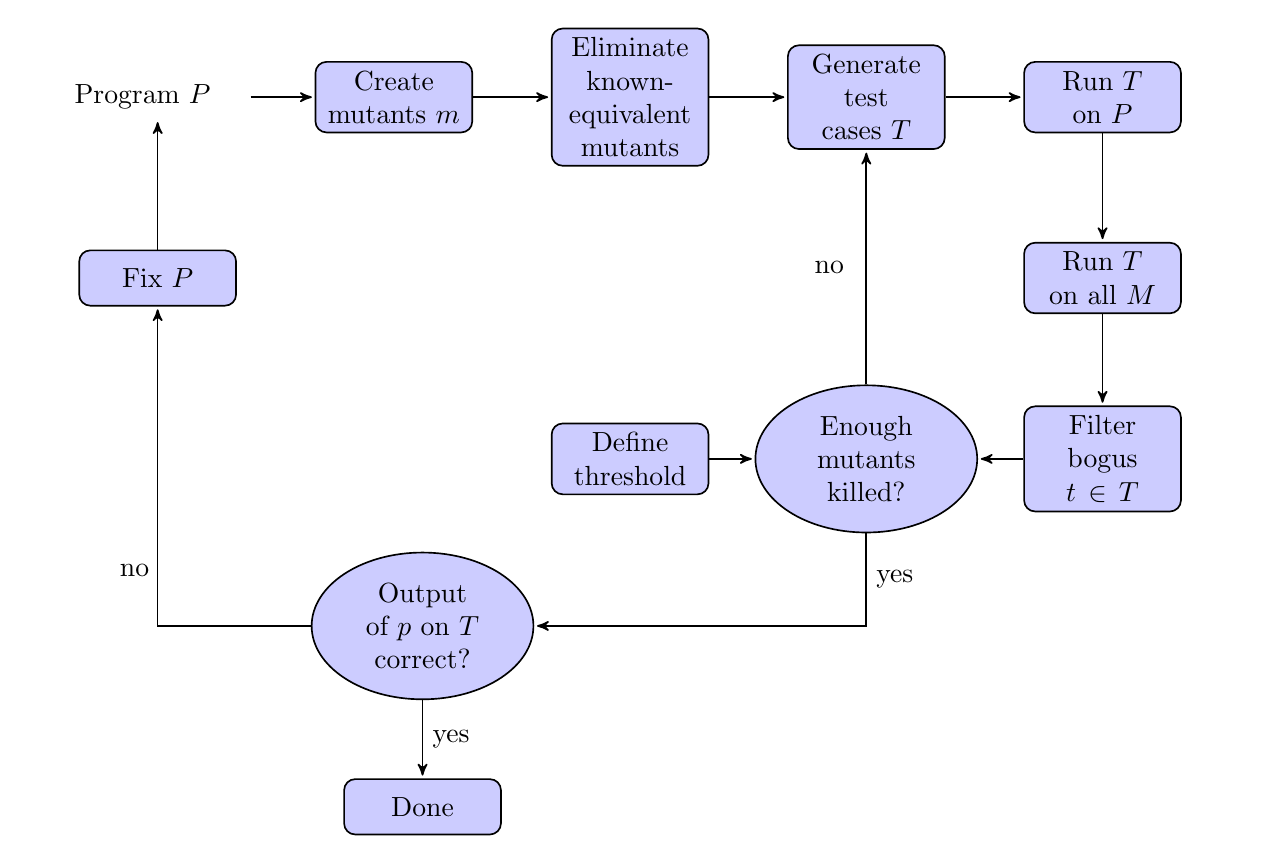
\begin{tikzpicture}[->,>=stealth',shorten >=1pt,auto,node distance=3cm,
                    text width=4em,
                    semithick,initial text=]
  \node[text width=6em] (p) {Program $P$};
  \node[block,right of=p] (create) {Create mutants $m$};
  \node[block,right of=create] (elim) {Eliminate known-equivalent mutants};
  \node[block,right of=elim] (gen) {Generate test cases $T$};
  \node[block,right of=gen] (runTonP) {Run $T$ on $P$};
  \node[block,below of=runTonP,yshift=2em] (runTonM) {Run $T$ on all $M$};
  \node[block, below of=runTonM,yshift=2em] (filter) {Filter bogus $t \in T$};
  \node[shape=ellipse, text centered, fill=blue!20, draw, text width=5em, left of=filter] (enough) {Enough mutants killed?};
  \node[block, left of=enough] (findThreshold) {Define threshold};
  \node[shape=ellipse, text centered, fill=blue!20, draw, text width=5em, below left of=enough,xshift=-10em] (correct) {Output of $p$ on $T$ correct?};
  \node[block, below of=correct,yshift=2em] (done) {Done};
  \node[block, below of=p,yshift=2em] (fixP) {Fix $P$};

  \path (p) edge node {} (create)
        (create) edge node {} (elim)
        (elim) edge node {} (gen)
        (gen) edge node {} (runTonP)
        (runTonP) edge node {} (runTonM)
        (runTonM) edge node {} (filter)
        (filter) edge node {} (enough)
        (findThreshold) edge node {} (enough)
        (correct) edge node {yes} (done)
        (fixP) edge node {} (p);
  \draw (correct) -| node[xshift=3em,yshift=2em] {no} (fixP); % no
  \draw (enough.north) -- node[xshift=2.5em] {no} (gen);
  \draw (enough) |- node[near start] {yes} (correct);
\end{tikzpicture}
\end{center}

\subsection*{Generating Mutants}

Now let's see how to generate mutants; this ties in to the
grammar-based material I talked about last time.  For mutation
testing, strings will always be programs.

\begin{defn}
Ground string: a (valid) string belonging to the language of the grammar (i.e. 
a programming language grammar).
\end{defn}

\begin{defn}
Mutation Operator: a rule that specifies syntactic variations of
strings generated from a grammar.
\end{defn}

\begin{defn}
Mutant: the result of one application of a mutation operator to a 
ground string.
\end{defn}

The workflow is to parse the ground string (original program), apply a
mutation operator, and then unparse.

It is generally difficult to find good mutation operators. One example
of a bad mutation operator might be to change all boolean expressions to
``true''. Fortunately, the research shows that you don't need many
mutation operators---the right 5 will do fine.

Some points:
\begin{itemize}[noitemsep]
\item How many mutation operators should you apply to get mutants? \emph{One.}
\item Should you apply every mutation operator everywhere it might apply? \emph{Too much work; choose randomly.}
\end{itemize}

\paragraph{Killing Mutants.} 
We can also define a mutation score, which is the percentage of mutants killed.

To use mutation testing for generating test cases, one would measure
the effectiveness of a test suite (the mutation score), and keep adding
tests until reaching a desired mutation score.

So far we've talked about requiring differences in the \emph{output}
for mutants.  We call such mutants {\bf strong mutants}.  We can relax
this by only requiring changes in the \emph{state}, which we'll call
{\bf weak mutants}.

In other words, 
\begin{itemize}[noitemsep]
\item \emph{strong mutation}: fault must be \emph{reachable},
\emph{infect} state, and \emph{\bf propagate} to output.
\item \emph{weak mutation}: a fault which kills a mutant need only be
\emph{reachable} and \emph{infect state}.
\end{itemize}
Supposedly, experiments show that weak and strong mutation require
almost the same number of tests to satisfy them.

Let's consider mutant $\Delta 1$ from above, i.e. we change
{\tt minVal = a} to {\tt minVal = b}. In this case:
\begin{itemize}[noitemsep]
\item reachability: unavoidable;
\item infection: need $b \neq a$;
\item propagation: wrong {\tt minVal} needs to return to the caller;
that is, we can't execute the body of the {\tt if} statement, so we
need $b > a$.
\end{itemize}
A test case for strong mutation is therefore $a = 5, b = 7$ (return
value = \textvisiblespace, expected \textvisiblespace), and for
weak mutation $a = 7, b = 5$ (return value = \textvisiblespace, expected
\textvisiblespace).

Now consider mutant $\Delta 3$, which replaces {\tt b < a} with {\tt 
b < minVal}. This mutant is an equivalent mutant, since {\tt a = minVal}.
(The infection condition boils down to ``false''.)

Equivalence testing is, in its full generality, undecidable, but we can always
estimate.

\subsection*{Program Based Grammars} 

The usual way to use mutation testing for generating test cases is by
generating mutants by modifying programs according to the language
grammar, using mutation operators.

Mutants are \emph{valid programs} (not tests) which ought to behave
differently from the ground string.

Mutation testing looks for tests which distinguish mutants from
originals.

\newpage
\paragraph{Example.} Given the ground string {\tt x = a + b},
we might create mutants {\tt x = a - b}, {\tt x = a * b}, etc.
A possible original on the
left and a mutant on the right:

\begin{minipage}{.5\textwidth} 
\begin{alltt}
int foo(int x, int y) \{ // original
  if (x > 5) return x + y;
  else return x;
\}
\end{alltt}
\end{minipage}\begin{minipage}{.5\textwidth}
\begin{alltt}
int foo(int x, int y) \{ // mutant
  if (x > 5) return x - y;
  else return x;
\}
\end{alltt}
\end{minipage}
~\\[3em]
In this example, the test case $\langle 6, 2 \rangle$ will kill
 the mutant, since it returns 8 for the original and 4 for the mutant,
while the case $\langle 6, 0 \rangle$ will not kill the mutant,
since it returns 6 in both cases.

Once we find a test case that kills a mutant, we can forget the
mutant and keep the test case. The mutant is then \emph{dead}.

\paragraph{Uninteresting Mutants.} Three kinds of mutants are uninteresting:
\begin{itemize}[noitemsep]
\item \emph{stillborn}: such mutants cannot compile (or immediately crash);
\item \emph{trivial}: killed by almost any test case;
\item \emph{equivalent}: indistinguishable from original program.
\end{itemize}

The usual application of program-based mutation is to individual statements
in unit-level (per-method) testing.

\bibliographystyle{alpha}
\bibliography{L15}
\end{document}
